\documentclass{report}

\usepackage{graphicx}
\usepackage{listings}

\usepackage{pdfpages} 

\usepackage{amsmath}
\usepackage{listings}
\usepackage{color} %red, green, blue, yellow, cyan, magenta, black, white
\definecolor{mygreen}{RGB}{28,172,0} % color values Red, Green, Blue
\definecolor{mylilas}{RGB}{170,55,241}


\title{\textbf{Advanced Telecommunications - Proxy}\\Owen Burke, 15316452}
\begin{document}

    \lstset{language=Matlab,%
    %basicstyle=\color{red},
    breaklines=true,%
    morekeywords={matlab2tikz},
    keywordstyle=\color{blue},%
    morekeywords=[2]{1}, keywordstyle=[2]{\color{black}},
    identifierstyle=\color{black},%
    stringstyle=\color{mylilas},
    commentstyle=\color{mygreen},%
    showstringspaces=false,%without this there will be a symbol in the places where there is a space
    numbers=left,%
    numberstyle={\tiny \color{black}},% size of the numbers
    numbersep=9pt, % this defines how far the numbers are from the text
    emph=[1]{for,end,break},emphstyle=[1]\color{red}, %some words to emphasise
    %emph=[2]{word1,word2}, emphstyle=[2]{style},    
    }

    \maketitle
    \section*{\hfil High-level description of the protocol design and implementation \hfil}
    The following implementation of a Proxy server is written in python 3.\\
    A Web proxy is a local server, which fetches items from the Web on behalf of a Web client instead of the client fetching them directly. 
    This allows for caching of pages and access control.\\
    The program should be able to:\\
    \textbf{1.} Respond to HTTP \& HTTPS requests, and should display each request on a management console. It should forward the request to the Web server and relay the response to the
    browser.\\
    \textbf{2.} Handle websocket connections.\\
    \textbf{3.} Dynamically block selected URLs via the management console.\\
    \textbf{4.} Efficiently cache requests locally and thus save bandwidth. You must gather timing and bandwidth data to prove the efficiency of your proxy.\\
    \textbf{5.} Handle multiple requests simultaneously by implementing a threaded server.\\\\

    \textbf{High-level description :}\\
    The first step was to establish a connection to the web browser so that the proxy could then forward on the requests to the end host.\\
    This was done by creating a socket that is bound to port 50000 on the localhost(127.0.0.1). Within the web browser's proxy settings, one can redirect all traffic through 
    any proxy of your choice, so these values must be provided.\\
    I then accept incoming connections on this socket, and for each connection is spool up a new daemon thread, starting with the handle\_browserConnection function.\\
    I also have the threads listening for a keyboard exception, in order for the user to provide input for blocking/unblocking hosts, etc.\\
    This "handle\_browserConnection" function does many of the essential operations such as determining whether the site is http/https, pulling out the information from the request
    about the end server, printing to the management console, determining whether the cached data is valid, etc.\\\\
    The design was then to have two different functions. One that deals with http traffic and another that deals with https.\\
    The http function is "forwardData" and this essentially just makes another socket that is connected to the end server, which we know from handle\_browserConnection. Then sends 
    the request to the server and then sends the response back to the connection we have made with the browser.\\
    The https function is "httpsForward" and this establishes a secure connection with the end server. In this function, when it receives a http connect request, it sends a http 200
    back to the browser connection, as a signal that we are ready to transmit (see https://en.wikipedia.org/wiki/HTTP\_tunnel).\\
    We then forward on the encrypted data from the browser to the server and vice versa. I believe this establishes a duplex stream allowing the proxy to handle web socket connections 
    (as the proxy correctly displays https://www.websocket.org/echo.html) (See figure 4).\\
    In terms of blocking hosts, when the user triggers the keyboard exception, by ctrl+c, they can either add or remove blocked hosts. Given that the proxy is threaded as mentioned before
    , host can be blocked/unblocked dynamically. This is implemented using a set as it has O(1)
    operations. Whenever the browser wants to communicate, the "handle\_browserConnection" function checks if the host is currently in the set. If it is not, the connection is performed
    as described above. If it is in the set, for http sites, a simple piece of html is returned to the browser saying the host is blocked. For https sites, the handshake isn't performed
    and the browser displays that the connection couldn't be established securely \textbf{(See figure 1 \& 2)}. In terms of design, I decided to block the host rather than the 
    specific URL, as this made more sense to me (to block all of www.nytimes.com rather than blocking www.nytimes.com/section/opinion and not blocking www.nytimes.com/section/business).\\

    
    For caching, whenever a request is made from the browser (as long as it is http, because https traffic cannot be cached due to encryption etc), the response is stored in a dictionary/hashmap where the key
    is the url from the request and the response is the associated value. If that request is made again, the proxy sends of the request to the server (with an If-Modified-Since header
    with the time stamp of the current cached value) and if the server responds with a 
    304, we know the value in the cache is up to date, and this data is sent back to the browser. If it is not a 304, the new data is read from the server into the cache, replacing the 
    old data and this is then sent back to the browser (the timestamp is also updated).\\

    Unfortunately, the caching doesn't work fully but you can see from the code that the foundation is there. You can see from the comments that certain aspects of the code 
    relates to caching. I am unsure as to why the time for the cache is greater than the time for the end server (as you can see from figure 3). To see the current state of the caching, you must uncomment these sections. Otherwise, comment them out to see the proxy work as expected just without caching.
    (See figure 3 for caching)\\
    Also, some times an connection refused exception will be thrown. I'm unsure as to why this is the case, however everything renders in the browser fine and all the links, etc work.\\\\

    



    \textbf{Code : }\\
    \lstinputlisting[language=Python]{proxy.py}





























    \begin{figure}[h!]
        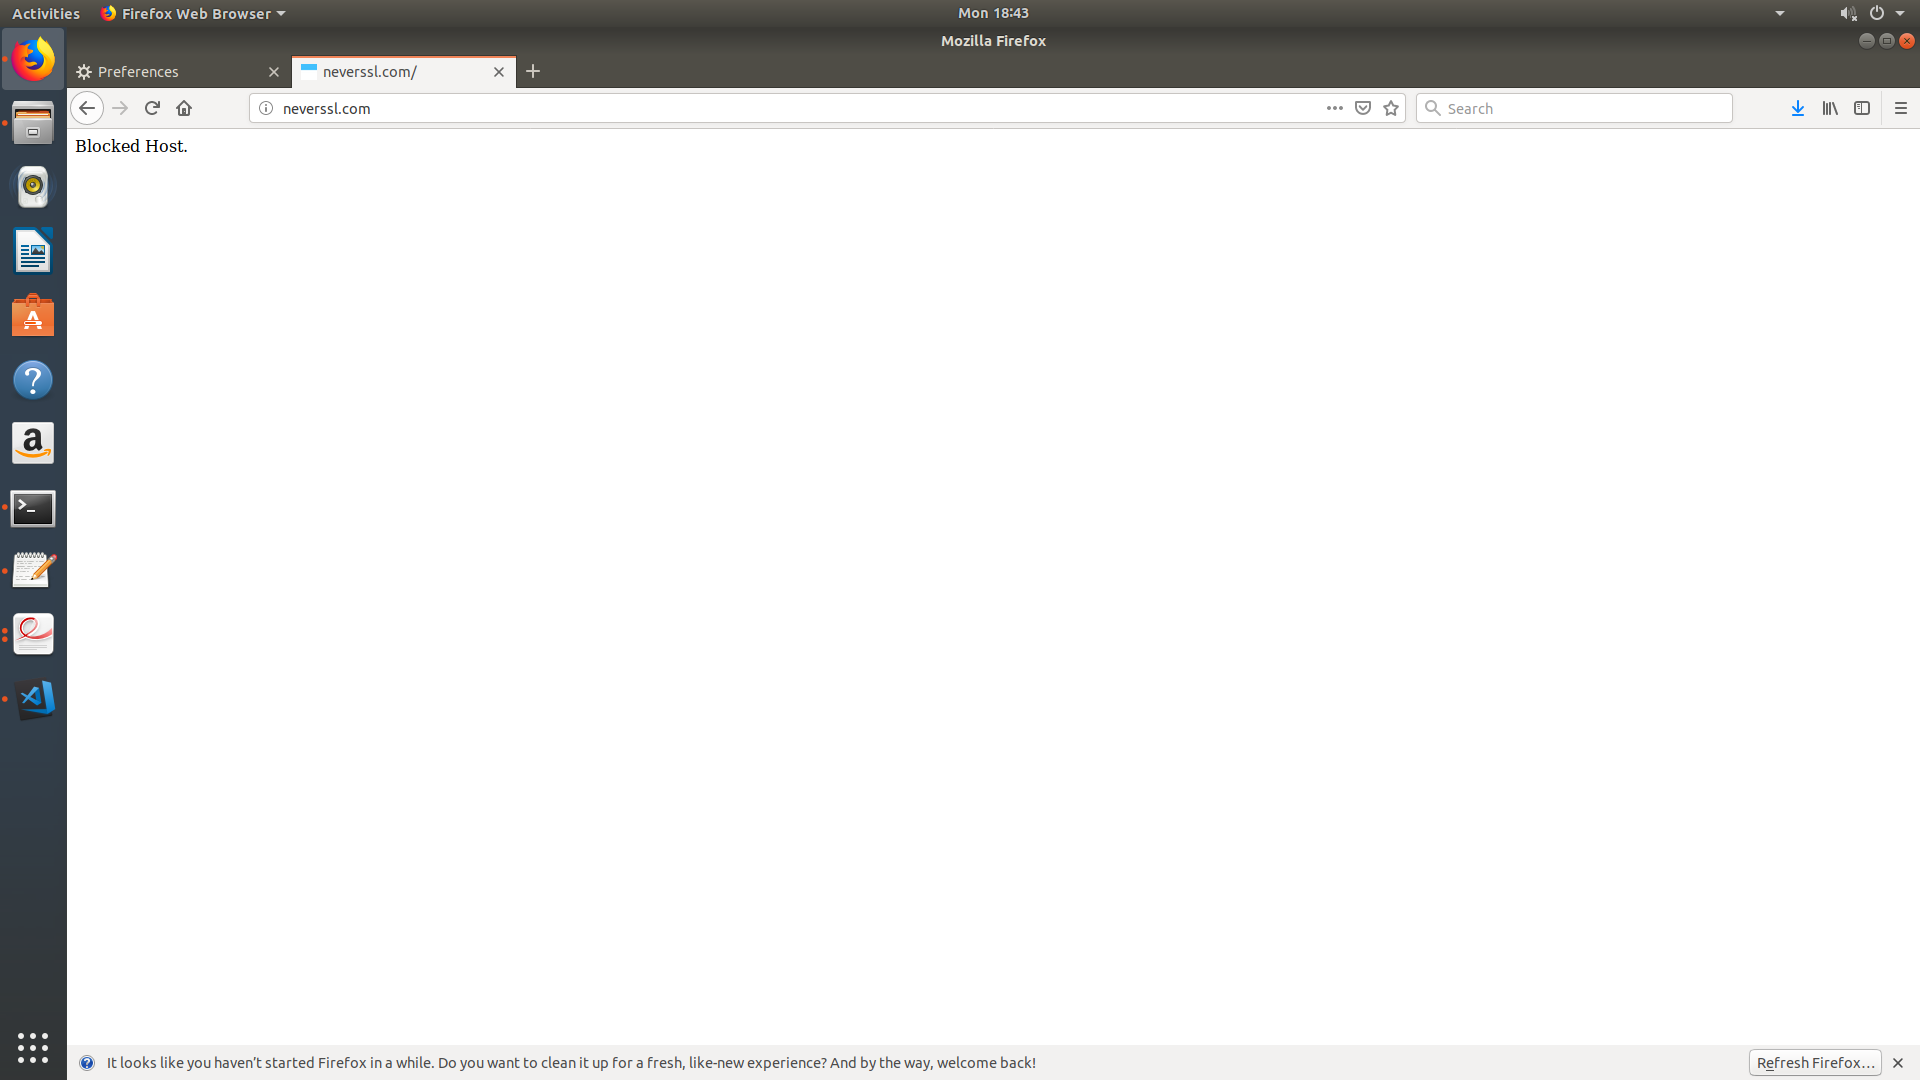
\includegraphics[width=\linewidth]{http_block.png}
        \caption{http blocking}
    \end{figure}

    \begin{figure}[h!]
        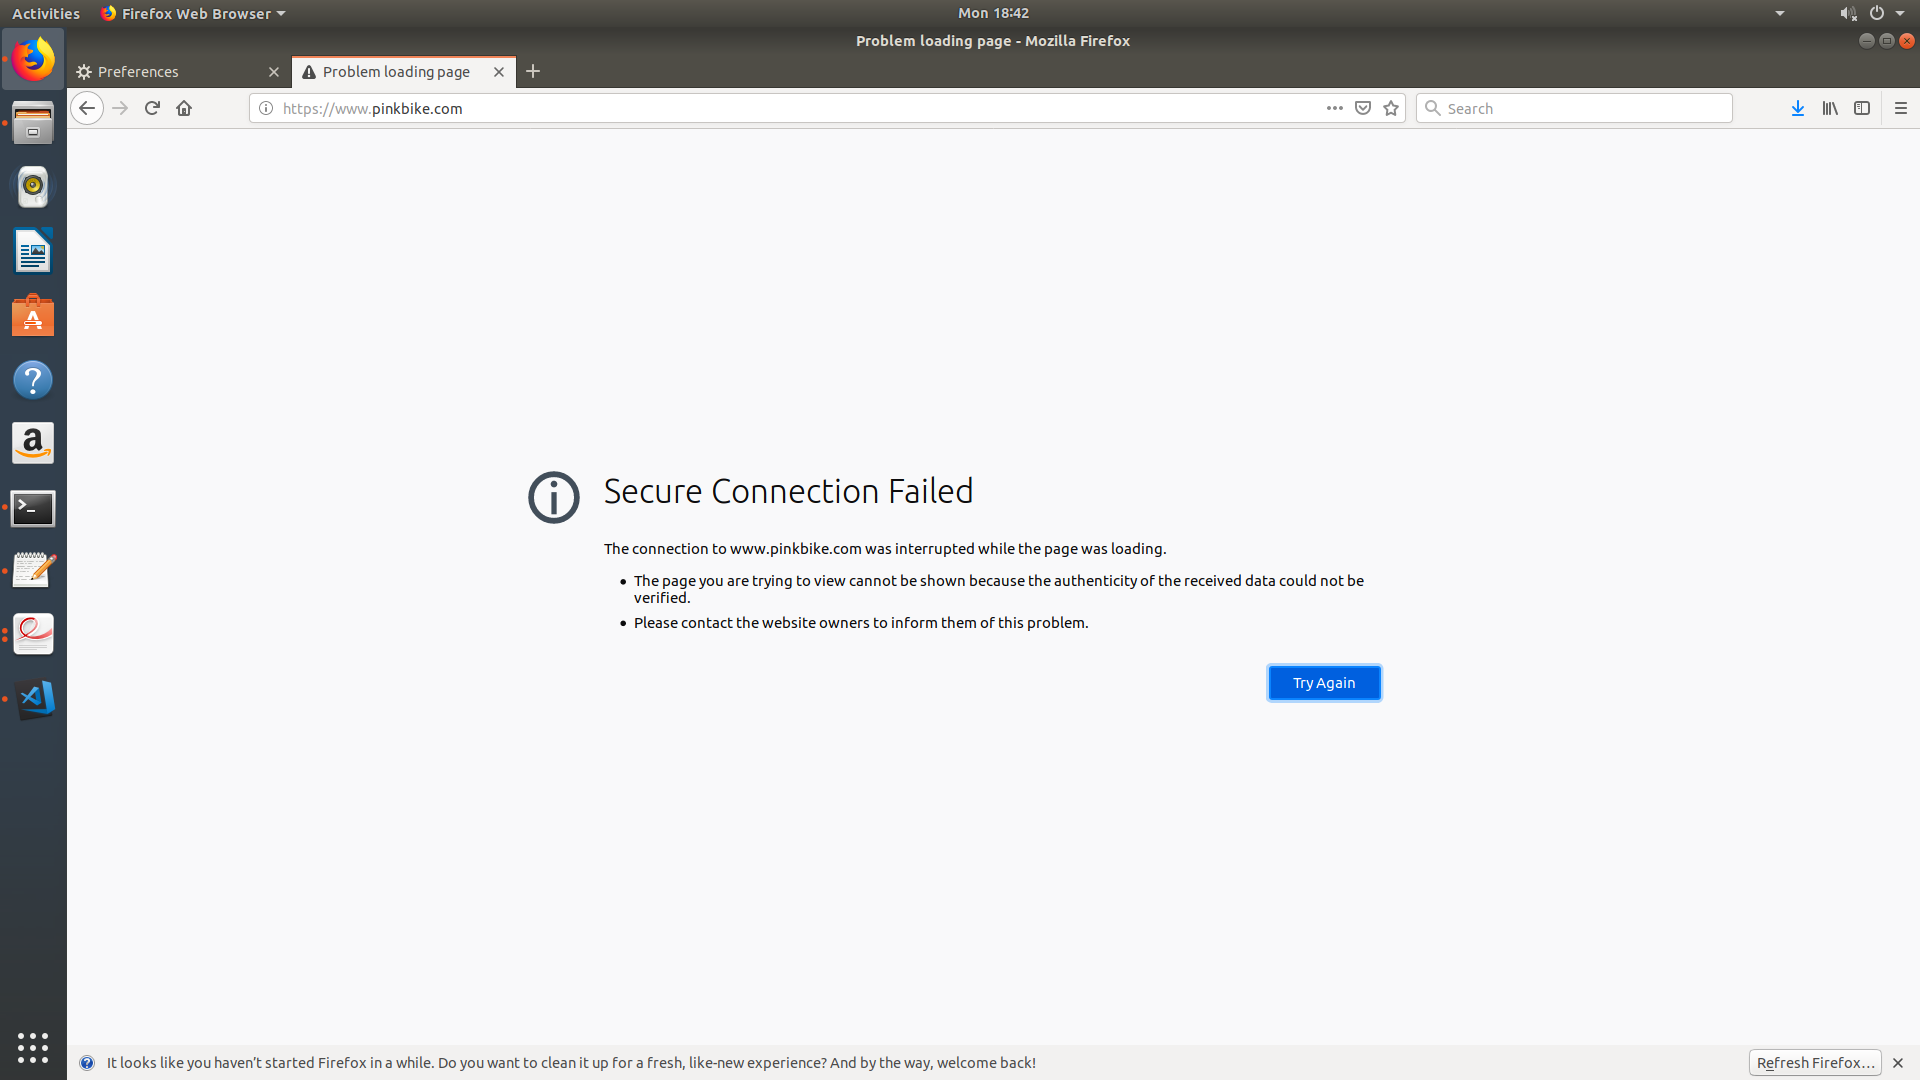
\includegraphics[width=\linewidth]{https_block.png}
        \caption{https blocking}
    \end{figure}

    \begin{figure}[h!]
        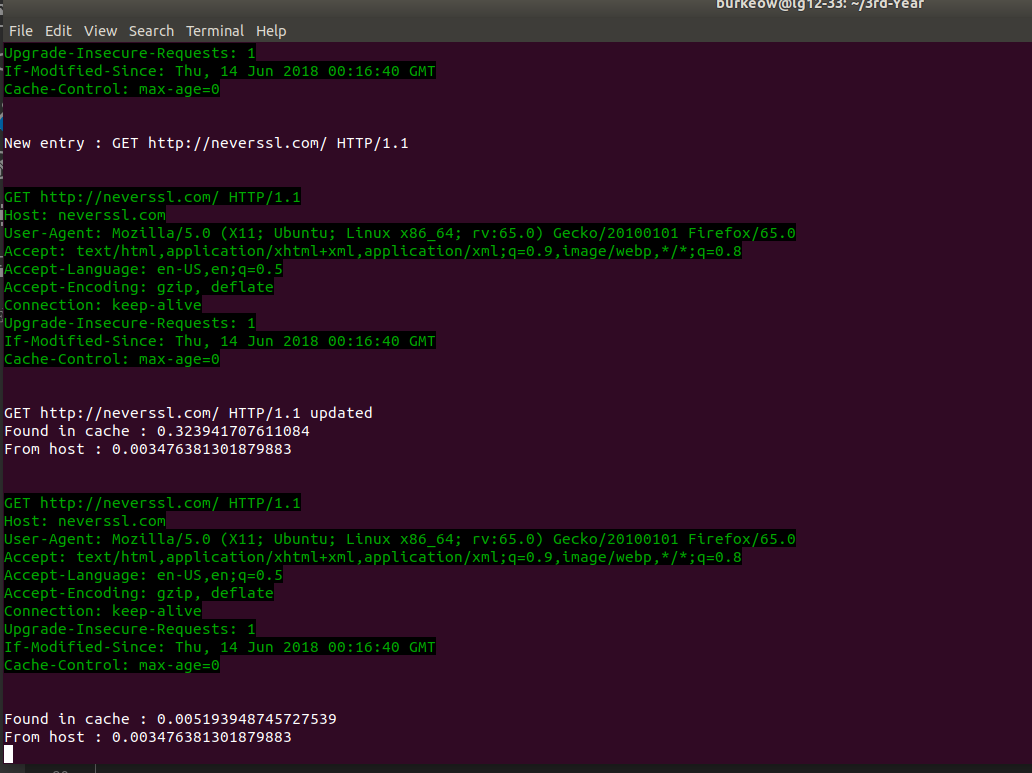
\includegraphics[width=\linewidth]{cache.png}
        \caption{caching}
    \end{figure}

    \begin{figure}[h!]
        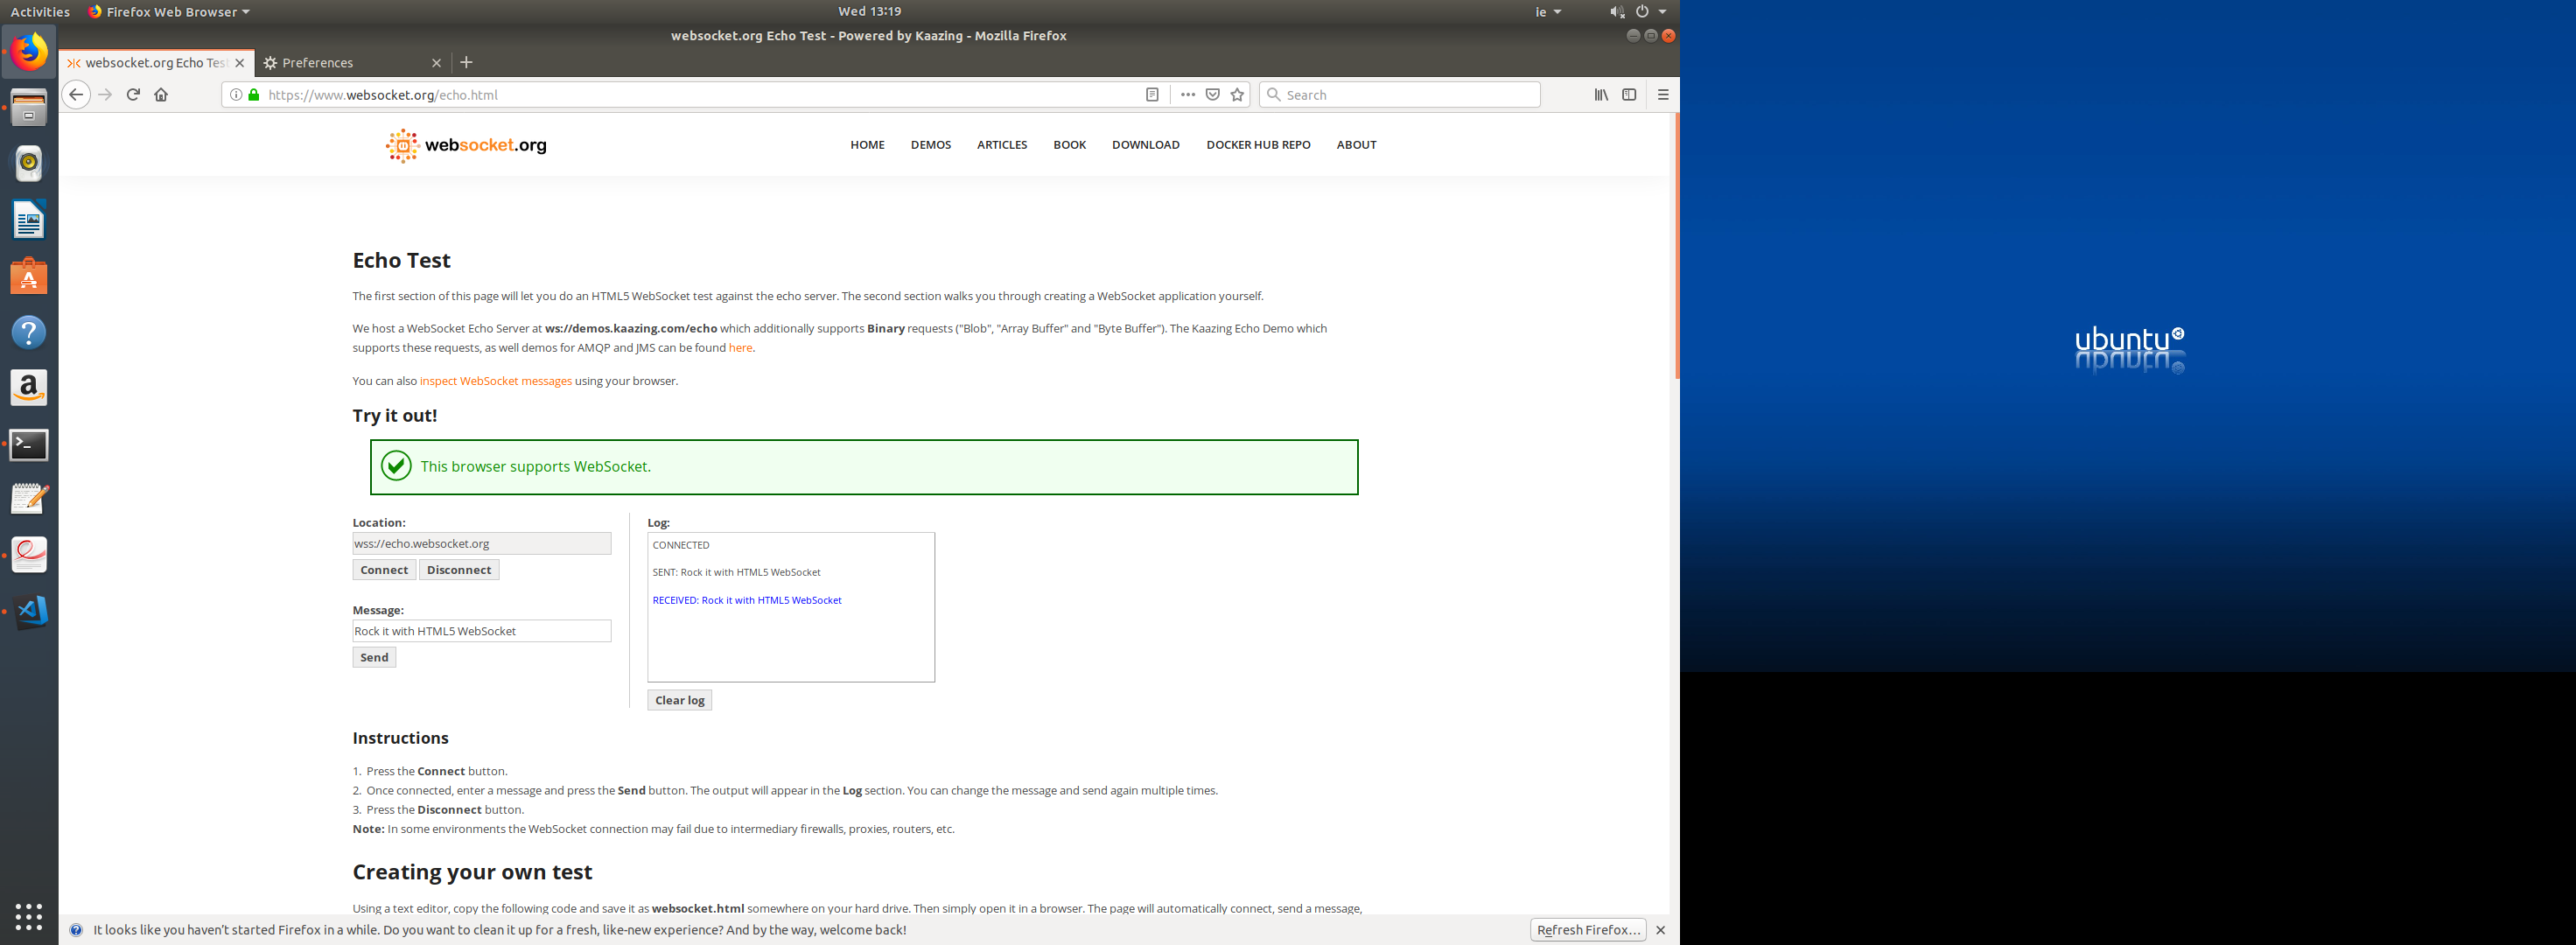
\includegraphics[width=\linewidth]{websockets.png}
        \caption{websockets}
    \end{figure}

\end{document}
